% https://tex.stackexchange.com/a/761452
\documentclass[tikz,border=5pt]{standalone}
\usetikzlibrary{nfold}
\makeatletter
\tikzset{%
    offset/.code=\tikz@addmode{%
        \pgfgetpath\tikz@temp
        \pgfsetpath\pgfutil@empty
        \pgfoffsetpath\tikz@temp{#1}
    }%
}%
\makeatother
% /tikz/insert path=<path>
% This key can be used inside an option to add something to the current path. This is mostly useful for defining styles that create graphic contents. 
\begin{document}
    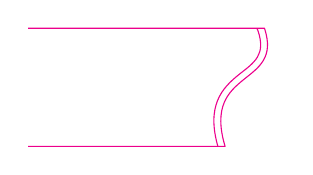
\begin{tikzpicture}[
        line join=round,
        double path/.style={
            insert path={
            .. controls ++(.25,-.75) and ++(-.3,1) .. (doubleend)
            }
        }
    ]
    \path (0, 1.5) coordinate (start)
        ++(3, 0 ) coordinate (doublestart)
        ++(-.5, -1.5) coordinate (doubleend)
        (0 ,0  ) coordinate (end)
    % negative timer to get a point before the start
        (doublestart) [double path] coordinate[pos=-.1] (doublestart-early)
    ;
    \draw[magenta]
    (start) -- (doublestart) [double path] -- (end)
        [path picture={
        \draw (doublestart-early) -- (doublestart) [offset=-2.5pt, double path];
        }]
    ;

    % How does it work: negative timer and turn key
    % \path (doublestart) [double path] node foreach \p in {-10, -9, ..., 10} [pos=\p/10, circle, fill=blue, inner sep=+.1pt]{};
    % \path[dashed, magenta] (doublestart) [double path] edge ([turn]0:.5);
    \end{tikzpicture}
\end{document}
